\chapter*{Introducción}\label{ch:introduccion}
\addcontentsline{toc}{chapter}{Capitulo 1. Introducción}

\section*{}
\addtocounter{section}{1}
\setcounter{subsection}{0}

\subsection{Área temática}
Los sitios de \textit{Community Question Answering} (CQA) brindan servicios que permiten a los usuarios formular y contestar preguntas sobre temas de cualquier índole. Miles de nuevas preguntas son subidas diariamente en sitios de CQA como Yahoo! Answers\footnote{Yahoo! Answers: \url{https://answers.yahoo.com/}. Último acceso: Octubre 2020.}, Stackexchange\footnote{Stackexchange: \url{https://stackexchange.com/}. Último acceso: Octubre 2020.}, Stackoverflow\footnote{Stackoverflow: \url{https://stackoverflow.com/}. Último acceso: Octubre 2020.}, o Quora\footnote{Quora: \url{https://www.quora.com/}. Último acceso: Octubre 2020.}. Estos son portales muy populares donde los usuarios suben diariamente una cantidad importante de preguntas de varios dominios para obtener respuestas de otros usuarios de la comunidad \citep{anuyah2017can}. Del análisis de sitios de CQA, puede observarse que muchas de las preguntas no están respondidas correctamente o no tienen respuestas específicas, ya que, en estas comunidades, hay típicamente un pequeño número de expertos entre la gran población de usuarios \citep{yang2013cqarank}. Por lo tanto, cuando un usuario realiza una pregunta, es de interés buscar si esa  misma interrogación ha sido formulada por otro usuario con anterioridad y para verificar que tenga la respuesta buscada. Por lo cual, el usuario podría leer las respuestas a dicha pregunta sin tener que esperar que la misma sea respondida. Esto no siempre es una tarea fácil, ya que podría darse la situación en la que la pregunta si exista previamente en el sitio y haya sido respondida y, sin embargo, esté formulada de una manera completamente diferente en el sentido léxico. Por esta razón, una correspondencia exacta (o casi exacta) no es aplicable. Consideremos el siguiente ejemplo, a partir del análisis de dos preguntas iguales: \textit{¿Cómo elijo una revista para publicar mi artículo?} y \textit{¿Dónde publico mi artículo?}\footnote{Traducción de las preguntas “How do I choose a journal to publish my paper?, Where do I publish my paper?” extraídas desde el conjunto de datos de Quora que se utilizará en el presente trabajo de tesis \url{https://data.quora.com/First-Quora-Dataset-Release-Question-Pairs}. Último acceso: Agosto 2018.}. Entre estas dos interrogaciones, existe apenas una superposición de palabras, sin tener en cuenta los \textit{stopwords}\footnote{En informática, se llama stopword a palabras que se filtran antes o después del procesamiento de datos del lenguaje natural \citep{leskovec2014mining}.}. Sin embargo, ambas preguntas tienen la misma respuesta, que referirá a revistas o sitios donde publicar un artículo científico.

\bigskip Con el fin de comparar dos preguntas, se establece entonces una medida de similaridad que se puede considerar como máxima cuando son idénticas y que es inversamente proporcional a las diferencias entre ellas \citep{lin1998information}. Pero teniendo en cuenta que una medida de similaridad de texto entre preguntas basada en características léxicas no las detectaría como preguntas iguales. Esto, deja en evidencia la necesidad de utilizar enfoques que, además, consideren características semánticas.

\bigskip A partir de lo expuesto anteriormente, puede decirse que la tarea de encontrar preguntas similares en sitios de CQA puede ser llevada a cabo por un Sistema de Recomendación. Los Sistemas de Recomendación (Recommender Systems o RS) son herramientas de software y técnicas que proveen sugerencias de ítems que es posible que los usuarios quieran utilizarlos \citep{ricci2011introduction}. Las sugerencias relacionan una variedad de procesos de toma de decisiones, como por ejemplo qué artículos comprar o qué música escuchar. El término general usado para denotar lo que los RS recomiendan a los usuarios es el vocablo “\textit{Ítem}”. Los ítems son objetos que pueden estar caracterizados por su valor o utilidad. El valor de un ítem puede ser positivo si el ítem es útil para el usuario y, negativo si no es apropiado. En este último caso, el usuario tomaría una mala decisión al seleccionarlo. A partir de la dinámica que se construye en los RS, las recomendaciones al usuario pueden ser personalizadas o no personalizadas. Las primeras, se basan en los comportamientos del usuario o en grupos de usuarios para encontrar sugerencias adecuadas a sus preferencias; las segundas, recomendaciones son inherentes a los ítems que el RS sugerirá. Cada una de estas estrategias de recomendación se elabora a partir de los diferentes conocimientos y datos recopilados por el sitio o el sistema donde el RS esté aplicado. Algunos ejemplos de tales aplicaciones incluyen la recomendación de libros, películas o ítems de compra de productos y/o servicios \citep{adomavicius2005toward}. En particular, para los sitios de CQA, los algoritmos de recomendación se aplican principalmente a elementos de texto. Este trabajo se centrará en ese tipo de recomendaciones, que pueden estar clasificadas dentro de RS basados en contenido de texto no personalizados, ya que las mismas están basadas únicamente en la estructura sintáctica y semántica de las preguntas existentes en los sitios de CQA. Los usuarios pueden navegar esas recomendaciones. Luego, pueden aceptarlas o no y, además, proveer inmediatamente o en un paso posterior, una retroalimentación explícita o implícita.

\bigskip A consecuencia de lo expuesto anteriormente, y sumado a que se dispone de un gran conjunto de datos, se diseñó e implementó una propuesta de arquitectura para utilizar Big Data con el fin de crear una medida de similaridad de texto que alimente a un RS especializado en la tarea de encontrar preguntas similares en sitios de CQA basado en análisis de contenido de texto. Este tipo de enfoque es necesario para procesar una gran cantidad de datos y, de esta manera, optimizar el procesamiento de los mismos, logrando velocidad y con la ventaja de poder aprovechar toda la variabilidad que provee un conjunto de datos de gran volumen. Luego de obtener esta nueva medida de similaridad, se realizará un análisis comparativo de la misma contra las medidas subyacentes utilizadas como entrada del método en cuestión.

\subsection{Tema específico}
\noindent Con el fin de dejar en claro el alcance de este trabajo, se toma como punto de partida el trabajo de investigación de la Universidad Tecnológica Nacional, Facultad Regional Rosario: “Comparative Analysis on Text Distance Measures Applied to Community Question Answering Data”, el cual se centra en el Paso 1 de de la secuencia de pasos (o \textit{pipeline}) que se describe en la Figura \ref{fig:pipeline}.
\bigskip
\begin{figure}[h!]
	\centering
	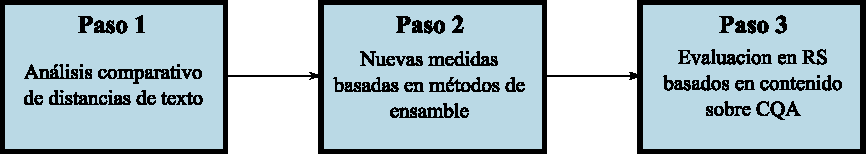
\includegraphics[width=0.9\linewidth]{5_introduccion/imagenes/pipeline}
	\caption{Pipeline para un RS basado en contenido de CQA y en una nueva medida de similaridad.}
	\label{fig:pipeline}
\end{figure}

Este proceso descrito en tres pasos, tiene como objetivo construir un RS basado en una medida novedosa de similaridad de texto. En el Paso 1 se realiza un análisis comparativo desarrollado a partir de medidas basadas en distancia, obtenidas a partir del análisis de texto, con el fin de evaluar RS a partir de grandes conjuntos de datos; en el Paso 2, a partir de los resultados arrojados por el Paso 1, se crea una nueva medida construyendo una matriz de similaridad basada en análisis de clustering, como una de las propuestas en los métodos \textit{Algoritmo de Particionamiento de Similitud basado en Cluster} (Cluster-based Similarity Partitioning Algorithm o CSPA) \citep{strehl33knowledge} y \textit{Clustering de Acumulación de Evidencias} (Evidence Accumulation Clustering o EAC) \citep{fred2005combining}. El método EAC, descrito en detalle más adelante, intenta mejorar la calidad de salida para una representación de similaridad basada en texto; por último, en el Paso 3 se debe aplicar la matriz de distancias obtenida en el Paso 2 en un RS basado en contenido, con el fin de evaluar su eficacia en sitios de CQA.

\bigskip Para tomar dimensión del volumen de datos que es necesario manejar con este enfoque basado en clustering, si, por ejemplo, tomáramos el conjunto de datos Quora (404301 pares de preguntas, es decir, 808602 preguntas totales), y quisiéramos generar una sola matriz de distancias cruzando par a par todas las preguntas entre sí, estaríamos calculando $\frac{n(n+1)}{2} = 326919001503$ distancias, donde $n = 808602$ y el resultado es la cantidad de elementos en la triangular superior. Esta matriz considera sólo una de las distancias de similaridad de texto del estado del arte, por lo cual si deseamos combinar varias medidas mediante un método de ensamble, deberíamos generar al menos una matriz por cada distancia del estado del arte, y luego usar las mismas para aplicar EAC, por lo cual estaríamos generando un número total de cálculos considerablemente mayor al que puede procesar una computadora clásica. Es necesario además tener en cuenta que las distancias pueden llegar a considerar características diversas entre sí, como morfología, sintaxis y semántica de los textos, lo cual añade complejidad y variedad al volumen considerado. Esto conlleva considerar una arquitectura Big Data, conjuntamente con optimización de código y técnicas de ejecución paralela entre un gran número de núcleos de procesamiento. Con respecto al espacio de almacenamiento, debe notarse que las matrices requieren doble precisión para la representación interna de cada uno de sus elementos (distancias), es decir 750 KB cuando están almacenados en un archivo, por lo cual, si consideramos la matriz ejemplificada anteriormente, necesitaríamos aproximadamente 12 TB para almacenarla, por lo cual, es necesario un esquema de almacenamiento optimizado para la implementación de este método. Con respecto a la velocidad de procesamiento, pruebas preliminares en un procesador potente brindan una estimación de alrededor de 3 años para completar el procesamiento. Con el problema planteado de esta forma, es indispensable aplicar un enfoque de Big Data para satisfacer los requerimientos de volumen, variedad y velocidad que requiere el contexto de análisis, de tal forma de brindar resultados veraces, y de esa forma cumplir con las premisas de las “V” del Big Data\footnote{Las “V” del Big Data refieren a Volumen, Variedad y Velocidad. También se consideran los conceptos de Valor y Veracidad con respecto al resultado de la aplicación del enfoque Big Data \citep{gandomi2015beyond}.}.

\bigskip Este trabajo de tesis apunta entonces a construir una medida de similaridad novedosa desde un enfoque Big Data, tal como se describe en el Paso 2 del pipeline, por lo cual es necesario crear un nuevo software basado en una arquitectura y patrones de Big Data, tomando como punto de partida el desarrollo del estado de arte.

\subsection{Objetivo general}
El presente trabajo de investigación tiene como objetivo construir una arquitectura Big Data que se aplique a grandes conjuntos de datos de preguntas de CQA y permita encontrar nuevas medidas de similaridad entre textos que puedan ser utilizadas en sistemas de recomendación.

\subsection{Objetivos específicos}
Se detallan a continuación, los objetivos específicos que son necesarios para lograr el objetivo principal.
\begin{enumerate}
	\item Identificar medidas de similaridad de texto existentes y un método efectivo de aplicación de las mismas en grandes volúmenes de datos.
	\item Diseñar y desarrollar una arquitectura Big Data para cálculo de similaridad en grandes matrices, que requerirá nuevas estrategias para recolectar, procesar y manejar grandes volúmenes de datos.
	\item Proponer una nueva medida que permita integrar las medidas de similaridad del estado del arte mediante una arquitectura de software basada en Big Data y que sea extensible a otras medidas
	\item Brindar conclusiones, pautas y recomendaciones para trabajar con medidas de comparación de textos en grandes volúmenes de datos en sitios de CQA utilizando arquitecturas basadas en Big Data.
\end{enumerate}